\documentclass[10pt,conference]{IEEEtran}

\usepackage{cite}
\usepackage{graphicx}
\usepackage{booktabs}
\usepackage{amsmath}
\usepackage{pgfplots}
\pgfplotsset{compat=1.17}
\usepackage[hidelinks]{hyperref}

\begin{document}

\title{BleedSense: Cross-Dataset Robustness for Surgical Blood Segmentation}

\author{
\IEEEauthorblockN{Riccardo Mazzi}
\IEEEauthorblockA{
Computer Vision and Cognitive Systems (CVCS) course, A.Y. 2025/2026 \\
University of Modena and Reggio Emilia (UNIMORE) \\
Supervisor: Dr. Livia Del Gaudio (AImageLab, TRAMIS project)
}
}

\maketitle

\begin{abstract}
Automatic hemostasis management in robotic surgery requires reliable segmentation of blood in the operative field. Models trained on a single surgical dataset, however, generalize poorly to other datasets with different visual characteristics. This work studies the problem on two public datasets, HemoSet (robotic surgery on a porcine model) and Rabbani et al. (gynecological laparoscopy on humans), confirming an asymmetric domain gap already observed in previous work from the research group, and systematically compares six families of strategies to reduce it: aggressive data augmentation, appearance/domain adaptation (Reinhard, FDA), multi-domain joint training (with and without balancing), ensembling of multiple architectures, an illumination-invariant input channel and feature-level style mixing (MixStyle), plus a test-time BatchNorm recalibration. Across three standard architectures (UNet, UNet++, DeepLabV3+, \texttt{resnet34} encoder), the most effective strategy is aggressive data augmentation, which improves cross-dataset robustness in both directions with no appreciable in-domain cost; combined with an ensemble of the three architectures, it yields the best overall result, and we analyze why the remaining strategies fall short of it.
\end{abstract}

\begin{IEEEkeywords}
semantic segmentation, domain generalization, cross-dataset robustness, surgical blood detection, data augmentation, domain adaptation
\end{IEEEkeywords}

\section{Introduction and Motivation}
\label{sec:intro}

Automating hemostasis management in robotic surgery -- identifying and controlling bleeding during the procedure -- requires, as a first step, reliable segmentation of blood in the endoscopic field of view. This project is part of the TRAMIS research initiative, focused on real-time bleeding detection in robotic surgery; since real, annotated TRAMIS surgical data were not yet available at the time of this work, the study was conducted on two public reference datasets in the domain, used as proxies:

\begin{itemize}
\item \textbf{HemoSet} \cite{miao2024hemoset}: induced bleeding during teleoperated robotic surgery on a porcine model, 962 image-mask pairs, 10 subjects.
\item \textbf{Rabbani et al.} \cite{rabbani2022midl}: gynecological laparoscopy on human patients, 751 annotated images.
\end{itemize}

Previous work from the research group \cite{giusti2026report} had observed an \emph{asymmetric} performance drop when a model trained on one of the two datasets is evaluated on the other: HemoSet$\rightarrow$Rabbani shows a strong general performance drop, while Rabbani$\rightarrow$HemoSet shows a marked increase in false positives (non-hemorrhagic regions segmented as blood).

\textbf{Project goal}: to quantify this asymmetry rigorously and reproducibly, and to systematically study which strategies actually increase the cross-dataset robustness of segmentation models, comparing multiple experimental conditions without the constraint of converging on a single solution.

\section{Related Work}
\label{sec:related}

Segmentation models for surgical and medical imaging are well known to generalize poorly across acquisition setups, instrumentation, and patient populations -- a domain gap that is especially acute for a visually heterogeneous, rare target such as intraoperative bleeding. HemoSet~\cite{miao2024hemoset} and the dataset of Rabbani et al.~\cite{rabbani2022midl} are, to our knowledge, the two public benchmarks for this specific task, respectively covering robotic surgery on a porcine model and human gynecological laparoscopy, each evaluated with its own protocol (IoU/F1/Hausdorff Distance, and IoU/F-Score); a first quantification of the asymmetric cross-dataset gap between the two -- the problem this work addresses -- was reported in an unpublished prior student project~\cite{giusti2026report}, which we use only as a starting reference point for that observation.

Two broad, architecture-agnostic families of techniques have been proposed to close such domain gaps without redesigning the network. The first acts at the appearance level, aligning low-level image statistics between source and target domains: explicit color transfer~\cite{reinhard2001color}, or exchanging low-frequency Fourier amplitude components while preserving phase (FDA)~\cite{yang2020fda}. The second acts at the feature level inside the network: MixStyle~\cite{zhou2021mixstyle} mixes encoder feature statistics across batch samples during training, while test-time BatchNorm recalibration (AdaBN)~\cite{li2016adabn} instead adapts normalization statistics to the target domain at inference, with no retraining. Separately, Su et al.~\cite{su2023aaai} show that a sufficiently varied data augmentation policy can itself act as an effective, architecture-free single-source domain generalization strategy -- a finding our own results corroborate. A more structural alternative is explicit style-content disentanglement, pursued by Teevno et al.~\cite{teevno2024cbms} for endoscopic segmentation and, in the same prior student project mentioned above~\cite{giusti2026report}, via a boundary-aware Transformer architecture; both require dedicated architectural components rather than only training-time interventions.

This work addresses a distinct question from all of the above: rather than proposing a new architecture, we systematically test which of the simpler, purely training-time interventions -- augmentation, appearance transfer, joint training, and ensembling -- actually improve cross-dataset robustness for this task, and why some succeed while others do not.

\section{Approach}

\subsection{Datasets and Splits}

HemoSet consists of 962 image-mask pairs from 10 subjects (pigs); we use a Stratified Group K-Fold split into 5 folds, with the subject as the group, to avoid the same animal appearing in both training and validation within the same fold. Rabbani consists of 751 images/masks with a fixed 70/15/15 split (train/val/test, seed 42), reused identically across all phases of the project.

\subsection{Architectures and Training Protocol}

We use three standard architectures via \texttt{segmentation\_models\_pytorch}, all with the same \texttt{resnet34} encoder for a fair comparison: UNet, UNet++, and DeepLabV3+. Training uses a combined Dice+BCE loss, the AdamW optimizer (lr $10^{-4}$), a \texttt{ReduceLROnPlateau} scheduler, batch size 8, $256\times256$ images, and the full dataset for each split. Early stopping on validation Dice is used (patience 8, cap of 40 epochs) -- we empirically verified, across all 87 Phase 1--4 runs, that this budget was sufficient for convergence (only 2/87 runs reached the cap, both with a residual improvement below 0.01 Dice). The exact same configuration is used for every condition compared, to isolate the effect of the single variable under study.

\subsection{Metrics and Evaluation Protocol}

We report Dice, IoU, Precision, Recall, F1, and HD95 (95th-percentile Hausdorff Distance). This set fully covers the metrics used in the original papers of both datasets, with HD95 preferred over the maximum HD because it is less sensitive to single-pixel outliers. A model trained on HemoSet is evaluated in-domain on the validation fold and cross-dataset on the fixed Rabbani test set; a model trained on Rabbani is evaluated in-domain on its own fixed test set and cross-dataset on the whole of HemoSet (never seen during training). We note that this makes the two datasets' results statistically asymmetric: HemoSet figures are mean $\pm$ standard deviation over 5 folds, while Rabbani (which has no natural grouping variable to fold over) contributes a single run -- Rabbani numbers should therefore be read with correspondingly more caution.

\section{Results}

\subsection{Baseline and Domain Gap Asymmetry}
\label{sec:results-a}

The three architectures, trained separately on the two datasets with minimal augmentation, confirm and quantify the asymmetry: for HemoSet$\rightarrow$Rabbani, mean Dice drops by about 70\% relative (0.745 $\rightarrow$ 0.217), with HD95 rising from $\sim$29px to $\sim$130px, driven by a collapse in recall (0.76 $\rightarrow$ 0.19): the model becomes too conservative on the target domain, missing most of the actual blood. For Rabbani$\rightarrow$HemoSet, the drop is more contained (0.684 $\rightarrow$ 0.585) but precision collapses (0.74 $\rightarrow$ 0.50) while recall stays high -- consistent with the original observation about false positives. The three architectures behave very similarly under every condition: none resolves the domain gap on its own. These baseline numbers are quantitatively consistent with the zero-shot estimates reported in~\cite{giusti2026report} (Dice 0.29 and 0.56 respectively) despite different splits and hyperparameters, which we take as a sanity check on our own measurements rather than a direct comparison.

\subsection{Data Augmentation, Appearance Adaptation, Joint Training}
\label{sec:results-b}

An ``aggressive'' augmentation (hue/saturation, gamma, blur, noise, JPEG compression, via Albumentations) improves cross-dataset robustness across all three architectures in both directions, at almost no in-domain cost (HemoSet$\rightarrow$Rabbani: 0.217 $\rightarrow$ 0.321, +48\% relative; Rabbani$\rightarrow$HemoSet: 0.585 $\rightarrow$ 0.601). Reinhard color transfer~\cite{reinhard2001color} and FDA~\cite{yang2020fda}, applied using unlabeled target-domain images, help the more critical direction (HemoSet$\rightarrow$Rabbani: 0.217 $\rightarrow$ 0.263 and $\rightarrow$0.242 respectively) but at a non-negligible in-domain cost (Rabbani in-domain: 0.684 $\rightarrow$ 0.611 with Reinhard) and do not beat aggressive augmentation. We hypothesize that, unlike augmentation (probabilistic, applied with some probability per image), adaptation here is always active during training: the model never sees the ``clean'' appearance of its own source domain, and ends up split between two styles instead of properly consolidating one with variations. Fig.~\ref{fig:augmentation} illustrates two independently-sampled draws of the aggressive policy on representative training images, to make concrete what is actually being varied beyond what the metrics alone convey.

% TODO: generate with `python visualize_augmentation.py` on the cluster, then
% copy results/qualitative/augmentation_example*.png into this Overleaf project's figures/ folder.
\begin{figure*}[t]
\centering

\includegraphics[width=0.95\textwidth]{figures/augmentation_example1.png}\\[2pt]

\includegraphics[width=0.95\textwidth]{figures/augmentation_example2.png}
\caption{Two representative HemoSet training images (left) alongside two independently-sampled draws of the aggressive augmentation policy (hue/saturation, gamma, blur, noise, JPEG compression, plus geometric flips) applied to each. The stochastic, per-sample nature of the policy is visible: the two draws for the same image differ from each other.}
\label{fig:augmentation}
\end{figure*}

Training on the union of HemoSet and Rabbani (joint training, with separate held-out test sets) was not a solution: no systematic benefit on HemoSet, and a systematic drop on Rabbani (0.684 $\rightarrow$ 0.636) caused by the size imbalance between the two datasets in the combined training set ($\sim$59\% HemoSet vs $\sim$41\% Rabbani). A domain-balanced sampling scheme (\texttt{WeightedRandomSampler}, $\sim$50/50 per batch) recovers only about half of the drop (0.636 $\rightarrow$ 0.656), without making joint training competitive with the other strategies.

\subsection{Ensemble of the Three Architectures}

As an additional methodological choice of our own, we ensembled the three architectures' predictions at zero additional training cost, simply averaging the sigmoid probabilities of the already-trained aggressive-augmentation checkpoints. The result beats the best single model on all four tested conditions, with modest but systematic, exception-free gains (e.g., HemoSet$\rightarrow$Rabbani: 0.337 best single model $\rightarrow$ 0.343 ensemble; Rabbani$\rightarrow$HemoSet: 0.615 $\rightarrow$ 0.623). This is consistent with the standard ensembling rationale: errors made independently by architecturally different models tend to disagree and partially cancel out when their probabilities are averaged, while the shared, correct signal is reinforced.

A practical caveat is worth noting given this project's real-time motivation (Section~\ref{sec:intro}): the ensemble triples inference cost (three forward passes instead of one) relative to a single model. This is a favorable trade-off for the offline evaluation performed here, but a deployed real-time bleeding-detection system would need to weigh the modest gains reported above against this added latency, or fall back to aggressive augmentation alone -- which is already the single most effective and cheapest strategy tested -- if strict real-time constraints apply.

\subsection{Comparative Summary}

Table~\ref{tab:summary} reports the mean over the three architectures for each strategy; full per-architecture results are in the supplementary materials.

\begin{table*}[t]
\centering
\caption{Mean Dice and HD95 (pixels) by strategy and evaluation condition, averaged over the 3 architectures.}
\label{tab:summary}
\small
\begin{tabular}{lcccccccc}
\toprule
& \multicolumn{2}{c}{HemoSet (in-dom.)} & \multicolumn{2}{c}{Rabbani (in-dom.)} & \multicolumn{2}{c}{H$\rightarrow$R (cross)} & \multicolumn{2}{c}{R$\rightarrow$H (cross)} \\
\cmidrule(lr){2-3} \cmidrule(lr){4-5} \cmidrule(lr){6-7} \cmidrule(lr){8-9}
Strategy & Dice & HD95 & Dice & HD95 & Dice & HD95 & Dice & HD95 \\
\midrule
Baseline (source-only)       & 0.745 & 28.9 & 0.684 & 48.0 & 0.217 & 129.9 & 0.585 & 58.7 \\
Aggressive augmentation      & 0.747 & 28.3 & 0.681 & 41.4 & 0.321 & 93.9  & 0.601 & 54.3 \\
Adaptation (Reinhard)        & 0.719 & 32.2 & 0.611 & 70.2 & 0.263 & 101.0 & 0.577 & 54.9 \\
Adaptation (FDA)             & 0.720 & 30.5 & 0.675 & 47.8 & 0.242 & 107.9 & 0.550 & 66.1 \\
Natural joint training       & 0.742 & 28.6 & 0.636 & 58.5 & n/a$^*$ & n/a$^*$ & n/a$^*$ & n/a$^*$ \\
Balanced joint training      & 0.739 & 31.3 & 0.656 & 55.2 & n/a$^*$ & n/a$^*$ & n/a$^*$ & n/a$^*$ \\
\textbf{Ensemble (3 arch.)}  & \textbf{0.770} & \textbf{24.6} & \textbf{0.706} & \textbf{39.6} & \textbf{0.343} & \textbf{91.5} & \textbf{0.623} & \textbf{49.6} \\
\bottomrule
\end{tabular}
\vspace{2pt}

\footnotesize{$^*$joint training is evaluated in-domain on both test sets, so there is no comparable cross-dataset condition for this row.}
\end{table*}

\begin{figure*}[t]
\centering
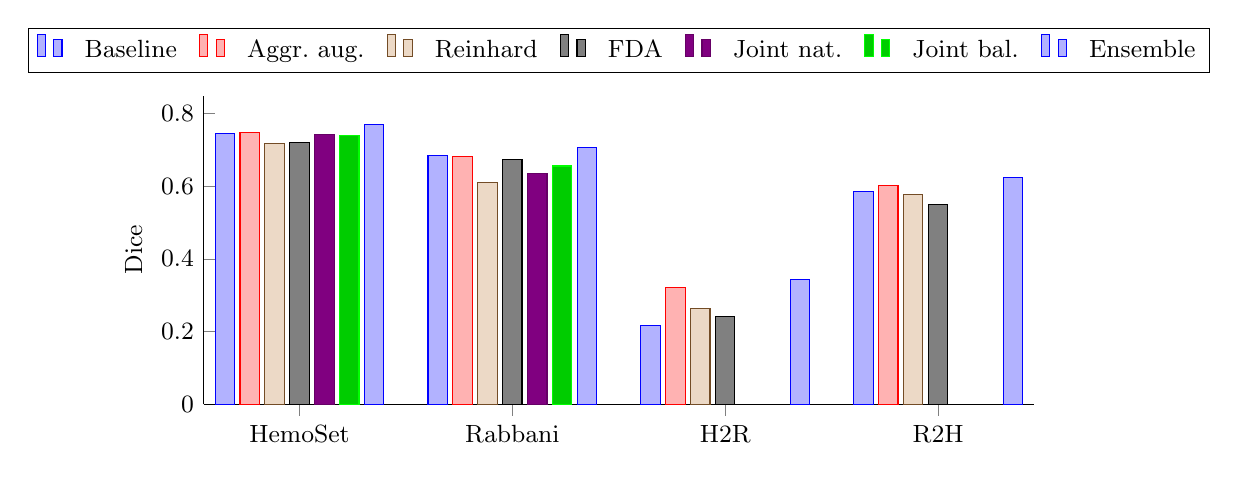
\begin{tikzpicture}
\begin{axis}[
    ybar,
    bar width=7pt,
    width=\textwidth,
    height=5.5cm,
    ymin=0, ymax=0.85,
    ylabel={Dice},
    ylabel style={font=\small},
    symbolic x coords={HemoSet,Rabbani,H2R,R2H},
    xtick=data,
    x tick label style={font=\small},
    y tick label style={font=\small},
    legend style={font=\small, at={(0.5,1.22)}, anchor=north, legend columns=7, column sep=6pt},
    enlarge x limits=0.15,
    axis lines*=left,
    clip=false,
]
\addplot coordinates {(HemoSet,0.745) (Rabbani,0.684) (H2R,0.217) (R2H,0.585)};
\addplot coordinates {(HemoSet,0.747) (Rabbani,0.681) (H2R,0.321) (R2H,0.601)};
\addplot coordinates {(HemoSet,0.719) (Rabbani,0.611) (H2R,0.263) (R2H,0.577)};
\addplot coordinates {(HemoSet,0.720) (Rabbani,0.675) (H2R,0.242) (R2H,0.550)};
\addplot coordinates {(HemoSet,0.742) (Rabbani,0.636)};
\addplot coordinates {(HemoSet,0.739) (Rabbani,0.656)};
\addplot coordinates {(HemoSet,0.770) (Rabbani,0.706) (H2R,0.343) (R2H,0.623)};
\legend{Baseline, Aggr.\ aug., Reinhard, FDA, Joint nat., Joint bal., Ensemble}
\end{axis}
\end{tikzpicture}
\caption{Mean Dice by strategy and evaluation condition (averaged over the 3 architectures). HemoSet/Rabbani = in-domain; H2R = HemoSet$\to$Rabbani (cross); R2H = Rabbani$\to$HemoSet (cross). Joint training bars are omitted in the cross-dataset columns (not applicable, see Table~\ref{tab:summary}).}
\label{fig:chart}
\end{figure*}

\textbf{Recommended configuration}: aggressive augmentation in training + ensemble of the three architectures at inference -- the only combination that improves cross-dataset robustness in both directions without penalizing in-domain performance.

\subsection{Qualitative Results}
\label{sec:qualitative}

Figures~\ref{fig:qual-h2r} and~\ref{fig:qual-r2h} show representative examples for each cross-dataset direction, comparing the ground-truth mask against the predictions of the source-only baseline, the aggressive-augmentation model, and the ensemble, overlaid on the original image. The baseline under-segmentation on HemoSet$\rightarrow$Rabbani (missed blood regions) and the over-segmentation on Rabbani$\rightarrow$HemoSet (false-positive regions) are visually apparent, and progressively mitigated by aggressive augmentation and further by the ensemble.

% TODO: generate with `python visualize_predictions.py` on the cluster, then
% copy results/qualitative/*.png into this Overleaf project's figures/ folder.
% Each figure stacks two examples to show the pattern is consistent, not cherry-picked;
% drop the second \includegraphics (and shorten the caption) if space runs short.
\begin{figure*}[t]
\centering

\includegraphics[width=0.95\textwidth]{figures/hemoset_to_rabbani_ex2.png}\\[2pt]

\includegraphics[width=0.95\textwidth]{figures/hemoset_to_rabbani_ex1.png}
\caption{HemoSet$\rightarrow$Rabbani, two examples: image, ground truth, baseline, aggressive augmentation, ensemble. The top example shows the baseline's characteristic under-segmentation (low recall), progressively recovered by aggressive augmentation and the ensemble.}
\label{fig:qual-h2r}
\end{figure*}

\begin{figure*}[t]
\centering

\includegraphics[width=0.95\textwidth]{figures/rabbani_to_hemoset_ex3.png}\\[2pt]

\includegraphics[width=0.95\textwidth]{figures/rabbani_to_hemoset_ex1.png}
\caption{Rabbani$\rightarrow$HemoSet, two examples: image, ground truth, baseline, aggressive augmentation, ensemble. The top example shows the characteristic over-segmentation (false positives) of this direction; the bottom example shows a cleaner case with only minor residual false positives.}
\label{fig:qual-r2h}
\end{figure*}

\section{Discussion}

\subsection{Why Augmentation Beats Adaptation and Joint Training}

The common factor behind the two less effective strategies -- always-active appearance adaptation, imbalanced joint training -- appears to be the lack of a mechanism that still preserves the model's exposure to the ``clean'' distribution of its own source domain during training. A light, probabilistic intervention on visual variety beats more targeted but always-active interventions on style, or simply mixing the data together. This is visually corroborated by the qualitative examples in Figs.~\ref{fig:qual-h2r}--\ref{fig:qual-r2h}: aggressive augmentation and the ensemble progressively recover the recall lost by the source-only baseline on HemoSet$\rightarrow$Rabbani, and reduce -- without fully eliminating -- the over-segmentation observed in the opposite direction.

\subsection{Three Further Extensions (Negative but Informative Outcome)}
\label{sec:extensions}

After identifying the recommended configuration, we attempted three additional original extensions:

\begin{enumerate}
\item \textbf{``Blood-index'' input channel} (ratio R/(R+G+B), in theory less sensitive to camera/illumination differences): slightly improves HemoSet$\rightarrow$Rabbani (0.321 $\rightarrow$ 0.331) but markedly worsens Rabbani$\rightarrow$HemoSet (0.601 $\rightarrow$ 0.526). The index, computed on raw pixels, carries over the white-balance differences between the datasets instead of ignoring them, becoming a shortcut feature specific to the source domain.
\item \textbf{MixStyle}~\cite{zhou2021mixstyle}: mixes the encoder's feature-map statistics between samples in the same batch. A diffuse but small degradation in both cross-dataset directions (0.217 $\rightarrow$ 0.203; 0.585 $\rightarrow$ 0.561), likely because it is applied too early in the encoder and because training batches remain single-domain in this setting, limiting the actual style diversity injected.
\item \textbf{Test-time BatchNorm recalibration} (AdaBN~\cite{li2016adabn}): recalibrates BatchNorm statistics on unlabeled target-domain images at inference time, with no additional training. Shifts the precision/recall trade-off in opposite directions in the two cross-dataset directions but net Dice does not improve in either direction (0.321 $\rightarrow$ 0.318; 0.601 $\rightarrow$ 0.570).
\end{enumerate}

None of the three beats the recommended configuration. The pattern is nonetheless informative: three very different mechanisms fail in the same way -- either introducing a shortcut specific to the source domain, or disturbing useful information without replacing it with something more transferable -- reinforcing the conclusion that aggressive augmentation + ensemble is not a local optimum that can be easily improved with light interventions, at least for this pair of datasets.

\section{Limitations and Future Work}

On the experimental design side, Rabbani's results rest on a single fixed 70/15/15 split rather than a cross-validated one; a classic $k$-fold cross-validation -- a plain random split into $k$ folds, without stratification, since no grouping variable analogous to HemoSet's subjects is available -- would provide a variance estimate comparable to HemoSet's 5-fold results, alongside a closer look at why one particular HemoSet subject is consistently harder to segment than the rest. On the methodological side, two refinements to the strategies already tested are natural next steps: applying appearance/domain adaptation with probability $<1$ instead of always-on, to check whether this alone explains the in-domain cost observed in Section~\ref{sec:results-b}, and combining it with aggressive augmentation to see whether the two effects compound rather than compete.

Two directions we did not explore trade simplicity for potentially larger gains at the cost of additional complexity: self-training with pseudo-labels on the target domain, and the style-content disentanglement or Transformer-backbone approaches discussed in Sections~\ref{sec:related} and~\ref{sec:extensions}. Finally, moving toward deployment, the ensemble could be extended across folds as well as architectures, and the recommended configuration should be re-evaluated on real TRAMIS data once available -- keeping in mind the domain-balancing lesson from our joint-training experiments, since mixing external datasets of very different sizes is not automatically beneficial without it.

\section{Conclusions}

This work systematically quantified the asymmetric domain gap between HemoSet and Rabbani, and compared six families of strategies for increasing the cross-dataset robustness of surgical blood segmentation models. Aggressive data augmentation proved to be the most effective and lowest-cost strategy among those tested; combined with an ensemble of three architectures, it produces the best overall result, with no additional training beyond what augmentation already requires. Three further extensions did not improve on this result, but their analysis supports the hypothesis that the key factor is preserving the model's exposure to the ``clean'' distribution of its own domain during training, rather than imposing invariance through signals or normalizations computed directly on the data.

\begin{thebibliography}{9}

\bibitem{miao2024hemoset} A.~J. Miao, S.~Lin, J.~Lu, F.~Richter, B.~Ostrander, E.~K. Funk, R.~K. Orosco, M.~C. Yip, ``HemoSet: The First Blood Segmentation Dataset for Automation of Hemostasis Management,'' \emph{International Symposium on Medical Robotics (ISMR)}, 2024.

\bibitem{rabbani2022midl} N.~Rabbani, C.~Seve, N.~Bourdel, A.~Bartoli, ``Video-based Computer-aided Laparoscopic Bleeding Management: a Space-time Memory Neural Network with Positional Encoding and Adversarial Domain Adaptation,'' \emph{Medical Imaging with Deep Learning (MIDL)}, 2022.

\bibitem{yang2020fda} Y.~Yang, S.~Soatto, ``FDA: Fourier Domain Adaptation for Semantic Segmentation,'' \emph{IEEE/CVF Conference on Computer Vision and Pattern Recognition (CVPR)}, 2020.

\bibitem{reinhard2001color} E.~Reinhard, M.~Ashikhmin, B.~Gooch, P.~Shirley, ``Color Transfer between Images,'' \emph{IEEE Computer Graphics and Applications}, 2001.

\bibitem{zhou2021mixstyle} K.~Zhou, Y.~Yang, Y.~Qiao, T.~Xiang, ``Domain Generalization with MixStyle,'' \emph{International Conference on Learning Representations (ICLR)}, 2021.

\bibitem{li2016adabn} Y.~Li, N.~Wang, J.~Shi, J.~Liu, X.~Hou, ``Revisiting Batch Normalization For Practical Domain Adaptation,'' \emph{arXiv:1603.04779}, 2016.

\bibitem{su2023aaai} H.~Su et al., ``Rethinking Data Augmentation for Single-Source Domain Generalization in Medical Image Segmentation,'' \emph{AAAI Conference on Artificial Intelligence}, 2023.

\bibitem{teevno2024cbms} M.~A. Teevno et al., ``Domain Generalization for Endoscopic Image Segmentation by Disentangling Style-Content Information and SuperPixel Consistency,'' \emph{IEEE International Symposium on Computer-Based Medical Systems (CBMS)}, 2024.

\bibitem{giusti2026report} F.~Giusti, F.~Marzo, Project report, Computer Vision and Cognitive Systems, UNIMORE, A.Y.~2025/2026.

\end{thebibliography}

\end{document}
